%% It is just an empty TeX file.
%% Write your code here.
\chapter{Communication System Test}



\section {ParSec Communication System}
Various signals transmitted in industrial environment have different requirements in terms of dependability. Let's consider a simple CCTV video transmission system. Each frame, even in low resolution solutions, consists of several hundred thousands pixels. The frame rate lies somewhere between 30 and 5 frames per second, depending on the requirements. Even multiple bit error in the compressed video information bitstream leads just to the corruption of some frames. Depending on the error rate and frame rate, such disturbance may not influence the correct service at all, just lowering the video quality. The system, despite some errors, still fulfills it's function.+

On the other hand the information flow between the control system and the nodes, placed on the robotic arms on the assembly line, consists in constant transmission of the coordinates of the destination and position of the arm. An error in such information can lead to the damage of manipulated objects or another catastrophic system failure.

Moreover, the quality of the signal propagation in such a rapidly changing environment is not constant. The error rate can significantly rise for a short time, but be relatively low otherwise. Spending time, power and resources on complex encoding and decoding may not be justified for the majority of the systems life time. The ability to adapt to the quality of the transmission would be just another advantage of well designed communication system.

In conclusion, the requirements of the industrial wireless system are diversified and need a configurable solution, that could offer a constantly high level of dependability while adapting to its environment and the use case. The high level of dependability means the coverage of the hardware faults in the first place, since they can even prevent the establishment and synchronization of the connection.

The goal of the ParSec project is to create a dependable, flexible and secure wireless communication system which meets all industrial automation requirements. It has to work with latencies below 1 ms and with very high noise level, serving many distributed clients at once. Moreover it has to deal with fading effects and potentially many reflections or even obstacles coming in the way of transmission and breaking it.

The ParSec communication system (shown in~\autoref{fig:ParSec}) consists of the MAC Layer processing, taking place within a standard processor, implemented mostly as software routines, followed by the a FEC unit and by a frame formatter. The last part is the baseband processor, which consists of mixed and analog signal processing and Radio Frequency unit. 

\begin{figure}[h]
\centering
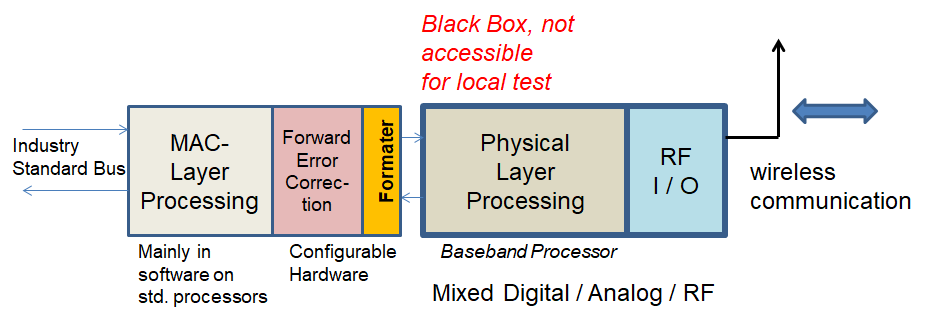
\includegraphics[width=0.65\textwidth]{figures/ParSec.png}
\caption{Block Diagram of the ParSec communiaction system}
\label{fig:ParSec}
\end{figure}

Both, the communication errors and soft errors due to transient faults in hardware, laying between FEC encoder and decoder, can be indivisible corrected thanks to ECC, as long as their number doesn't exceed the ECC correction capabilities. 

There are many techniques to improve the signal quality and make it resistant to fading effects due to multi-path signal propagation, poor signal-to-noise ratio or interferences, lowering the error rate. The known and used techniques involve Orthogonal Frequency Domain Multiplexing (OFDM) \cite{book:OFDM,art:OFDM}, Spread-Spectrum Communication \cite{art:spread-spectrum96,art:spread-spectrum97} or Ultra Wide-Band Frequency Communication \cite{book:ultra-wide08,book:ultra-wide04}. The OFDM technique would be suitable, but it ruquires many very fast AD converters~\cite{art:PSSS04}. The solution chosen for ParSec project is the Parallel Sequence Spread Spectrum (PSSS) technology~\cite{art:PSSS15,art:PSSS04,patent}. It provides comparable transmission quality as OFDM, without the cost of expensive AD converters.

The theory behind the creation of Error Correction Codes (ECC) has been presented in \autoref{sec:cod}. The detection and correction of single bit errors can be achieved using a simple Hamming code \cite{art:Hamming}. With Hsaio Code or extended Hamming Code the single error correction and double error detection is possible \cite{book:Fujiwara,art:Hsiao}. Unfortunately in such a noisy and harsh environment as industrial production site, there may be faults causing more than one or two bit flips in the data bit stream. For such purposes the multiple-bit correcting codes like Reed-Solomon code \cite{Redd-Solomon} or BCH Code \cite{BCH} are suggested. They typically require much more effort in  encoding and especially in decoding the information. They tend to be slower. There are also other methods to deal with correction of two-bit errors like \cite{Hosp, Varghese}. All these proposals lack a simple one-fits-all solution, that could be used and configured to the needs of the target system and it's environment.
The FEC is realized thanks to the Programmable Encoder Architecture (PENCA) designed by P. Pfeifer, firstly introduced in \cite{art:Pfeifer}, showed in~\autoref{fig:PENCA}. It is an answer to the strict requirements of the dependable communication systems. The core of the solution consists in the "honeycomb" structure of units. The units can be replaced by neighboring units in case of errors detected in one of them. The internal test can be performed automatically or on demand. After testing, the unit can be marked as faulty, once the test fails, and its functionality logically remapped into another unit. Both the input and output units are implemented in two copies, since they are single points of failure and in case of permanent fault detected wouldn't be able to get repaired without a spare. The control of the system is done through the microcode (secured with parity bits). But above all, the architecture can be configured to serve as different channel encoders, starting with the implementation of the single error correcting codes and ending with the multiple-bit error correcting codes or even cross-parity codes. It is done via generation of polynomials by each unit and sometimes even borrowing resources from neighboring units for more extended polynomial generations. Each unit being able to perform BCH generator polynomial length task up to 42 coefficients (34 BCH codes) or 65 coefficients (50 BCH codes) with borrowed resources.
 \begin{figure}[h]
 \centering
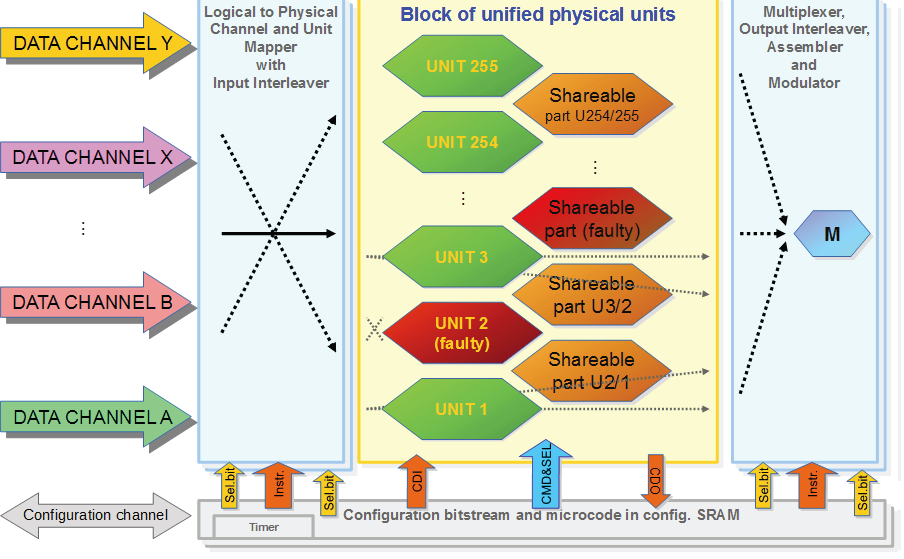
\includegraphics[width=0.25\textwidth]{figures/PENCA.png}
\caption{Basic scheme of the new dependable PENCA architecture~\cite{art:Pfeifer}}
\label{fig:PENCA}
\end{figure}
The hard errors due to permanent faults in hardware modules require special treatment since they can even prevent the synchronization of transceiver and receiver and therefore cannot be so easily corrected by FEC. Since permanent faults don't disappear, they also need special repair mechanism, which often means a doubling of the unit or its parts. The fault diagnosis proves to be complicated, especially in the mixed signal and analog parts, moreover when the access to this parts is limited. When an IP is shipped as a "black box" and there is no possibility to implement any internal DfT techniques, some sort of external test is required. 

\section{Functional Shorts Concept}
Thanks to the ECC, a precise detection of error positions in the received bit stream is possible, as long as the error count doesn't exceed its correcting capabilities. The idea behind the diagnostic test based on extended FEC functions is to use the existing FEC redundancy and detect not only soft errors and transmission errors, but also hard errors due to permanent faults. As mentioned in the~\autoref{sub:limits} the ECC can be used in hardware monitoring only if the input and output of the UUT are identical. Since the wireless communication is usually a duplex communication, every node happens to own both, the transmitter and receiver. They consist of complementary building blocks. Every modulator in transmitter is substituted with a demodulator in receiver, every encoder with decoder. The basic task of the receiver modules is to recreate the original information sent by transmitter, step by step, layer by layer. A diagnostic test would require to short the transmitter with receiver and systematically short the outputs of every module with the inputs of their corresponding module. With encoder and decoder in one closed system, it should be possible to detect the exact positions of errors in the bitstream and identify faulty units. The decoder would act as a response analyzer. In this way, the information leaving FEC encoder arrives at the input of FEC decoder, manipulated only by permanent faults in the shorted modules. The idea is presented in~\autoref{fig:Shorts}. 

\begin{figure}[h]
\centering
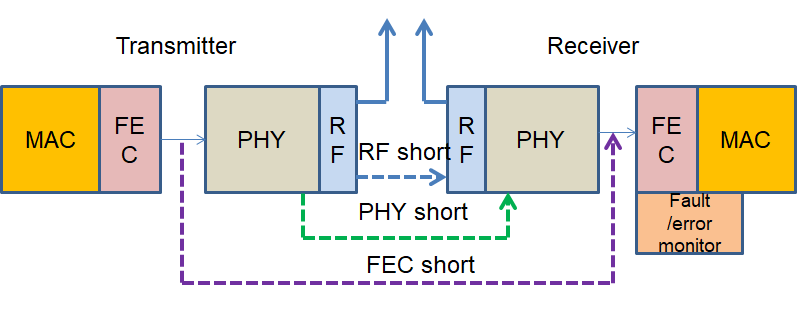
\includegraphics[width=0.65\textwidth]{figures/Shorts.png}
\caption{Transmitter and receiver shortcut idea for diagnostic test purposes}
\label{fig:Shorts}
\end{figure}

In order to conclude such test, the physical shorts need to be implemented. A simple multplexer demultiplexer pair with the common control logic would allow to choose between a normal functionality and shortened path. Additionally the test vectors need to be generated or stored in ROM. The fault detection occurs thanks to an extended decoder functionality, which signalizes, with a special ISERR output, if the current bit of the bit stream has been flipped or not. This functionality is also used during the normal data flow, to adjust the transmission parameters and adapt the FEC algorithm. A simple counter connected to this special output counts the number of bit flips in every block. This information can be used for channel quality estimation. 

The idea of functional shorts has been implemented into the Test Bench together with error injection capability and is shown in \autoref{fig:short_ena}. The injected error vector flips the chosen bits of the output of any module to simulate the possible effects of hardware faults on the processed information. The implementation lacks real modules, except from the encoder and decoder. Every other module is implemented as a simple delay in the digital information flow. The Air simulates the communication channel. There is also a programmable delay to variate the execution time of the test and to simulate the fact, that the number of clock cycles, needed for the information to pass from the encoder to decoder, is not constant.

\begin{figure}[h]
\centering
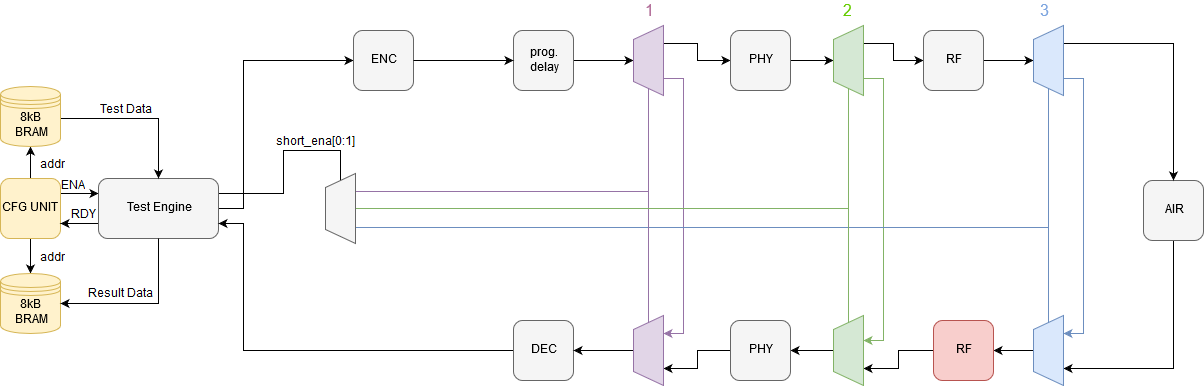
\includegraphics[width=\textwidth]{figures/Short_ena_err.png}
\caption{Implementation of functional shorts into the Test Bench}
\label{fig:short_ena}
\end{figure}

\subsection{Diagnostic test Procedure}
Let's assume, that the FEC decoder is fault-free and that every module owns some sort of repair ability. The erroneous unit would be the Radio Frequency unit of the receiver.
\begin{enumerate}
    \item Start the test by enabling the shortcut nr. 3, closing the test loop between transmitter and receiver
    \item Conclude the test by running all test vectors through the design, placing them on the inputs of FEC encoder, until the first occurrence of the ISERR set high
    \item Enable shortcut nr. 2
    \item Run test again and detect no errors, since the faulty unit is not in the test loop
    \item Run repair procedure on the transmitter RF unit
    \item Enable Shortcut nr. 2
    \item Run the test only to see the ISERR is high again
    \item Run repair procedure on RF unit of the receiver, revert the repair of the transmitter RF unit
    \item Start the test again to see no errors detected
\end{enumerate}

After running the test, all injected faults have been detected and the shorts system was able to identify the faulty unit. The number of injected faults have never exceeded the error correction capabilities of the decoder and the decoder was always assumed to be fault-free. Additionally the faults have been injected in random places, not necessarily corresponding to real permanent faults effects.

\section{Test of the BCH(1023,943) Encoder}
The PENCA architecture contains a BIST functionality, but let's assume a communication system having a simpler encoder/decoder pair. The tested encoder is a BCH encoder taking 943 payload bits and calculating 80 parity bits. The encoder is actually a part of the PENCA architecture, without any redundant test and configuration circuitry. The encoder consists of input shift register, a mesh of XOR gates for parity calculations and the counter to keep track on the number of input bits. When the counter reaches 943 bits, the output starts to send parity bits. Since the test bench developed during the project allows a test with wide range of frequencies, it may be possible to cause some delay faults in th encoder architecture and examine, how they influence the output bit stream. 

The encoder has been placed in the test bench and tested for maximum frequency. The result is shown in \autoref{tab:enc}.

\begin{table}[]
\begin{tabular}{@{}lllll@{}}
\toprule
UUT                       &mem\_width   &uut\_width &expected freq. &max. freq.\\ 
\midrule
isolated Encoder                  & 32          & 4      & $\sim$642 MHz & $\sim$500 MHz \\
not isolated Encoder              & 32          & 4      & $\sim$642 MHz & $\sim$326 MHz \\
\bottomrule
\end{tabular}
\centering
\caption{Test Encoder for max. frequency}\label{tab:enc}
\end{table}

The relatively low frequency is caused by the design placing inside the FPGA. The encoder is capable of running at least a double of 300 MHz, but it has been placed in a different clock domain in FPGA. This fact is favorable, since the test engine has been tested to work only until 500 MHz and it wouldn't be possible to cause any delay faults in the design, which is much faster then the test engine. It has been proven during the test of isolated encoder, which was surrounded by flip flops. The delay faults started to show up in the test engine logic by 500 MHz. The not-isolated version contains very long paths, which are perfect for simulating effects of delay faults. The frequency values are of course to be omitted, since they don't reflect the real values at all. 

The Encoder test was conducted with random data input. First clock cycle is reserved for the reset. After the reset is low, the input vector is shifted in serially. The output is hard-wired with the input when the payload bits are shifted in. After 943 payload bits, the input is set to zero and held that way till the end of the test, which means another 80 clock cycles, for the parity bits to be shifted out. The test consist in 300 test vectors. The frequency is changed by 100 MHz at a time until the test fails. The step is then lowered to 10 MHz and repeated from the last successful run. The step may be lowered as long as the synthesized frequencies allow or until a satisfying precision is achieved.

\autoref{fig:enc_1} represents the result of the failed test at apprx. 355 MHz. In half of the vectors (called blocks) the first parity bit is corrupted. When the counter, calculating the number of shifted bits, reaches the 943, the output should be switched to the parity bits. In all vectors, the output still forwards the input value, which is zero for all parity bits. In half of the vectors, since they are randomly distributed, the zero is accidentally the expected value, therefore the error gets masked.

\begin{figure}[h]
\centering
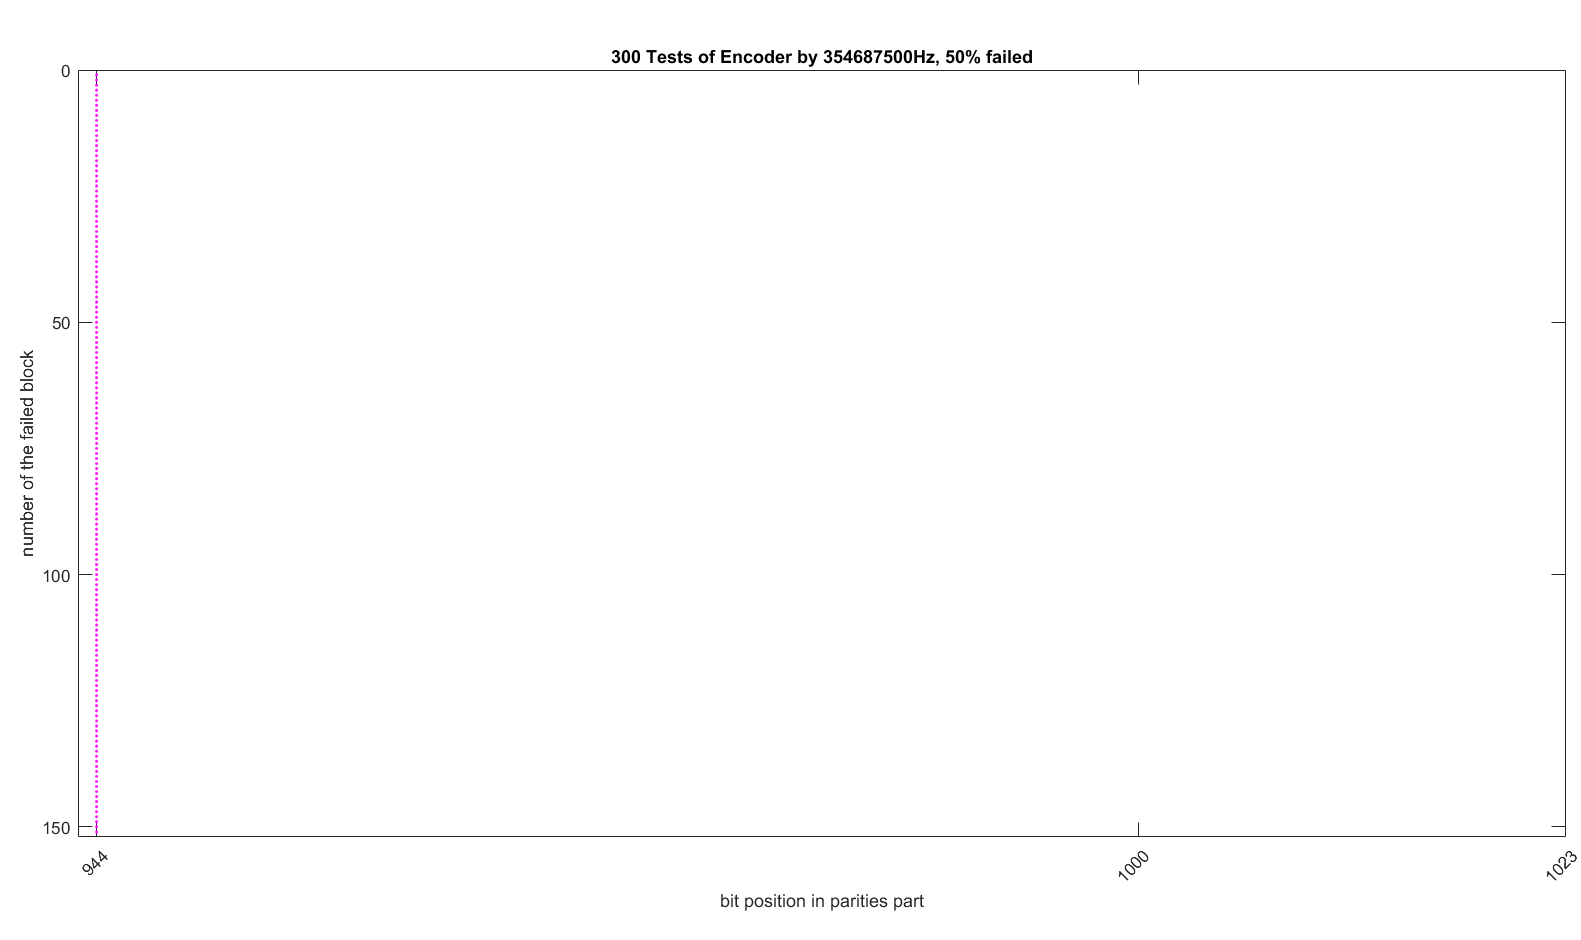
\includegraphics[width=\textwidth]{figures/test_ENC_1.png}
\caption{The result of failed Encoder test by 355 MHz}
\label{fig:enc_1}
\end{figure}

The further raise of the test frequency reveals another paths failing. The \autoref{fig:enc_2} shows the parity bits of the failed test. In addition to the 944th bit, there are more bits flipped in the parity part of the vector. There is no possibility, that the XOR gates, which are implemented as LUTs in the FPGA, fail at such a low frequency. The values from correctly calculated parity bits don't reach the input flip-flop of the test engine within the time frame. The number of bits correspond to the number of paths that fail at the same time, hence their net delays are comparable. The effect may seem impossible in the real hardware, but multiple bit flips in encoder architectures have been reported \cite{art:Dicorato}, based on Hsiao-Code encoder architecture. The cause of the error are faulty XOR gates with big fan-outs, taking part in computation of more then one parity bit. The suggested solution involves use of more XOR gates, to avoid such situations. The overhead for Hsiao-Code encoder seems to be around 10\% in logic.

\begin{figure}[h]
\centering
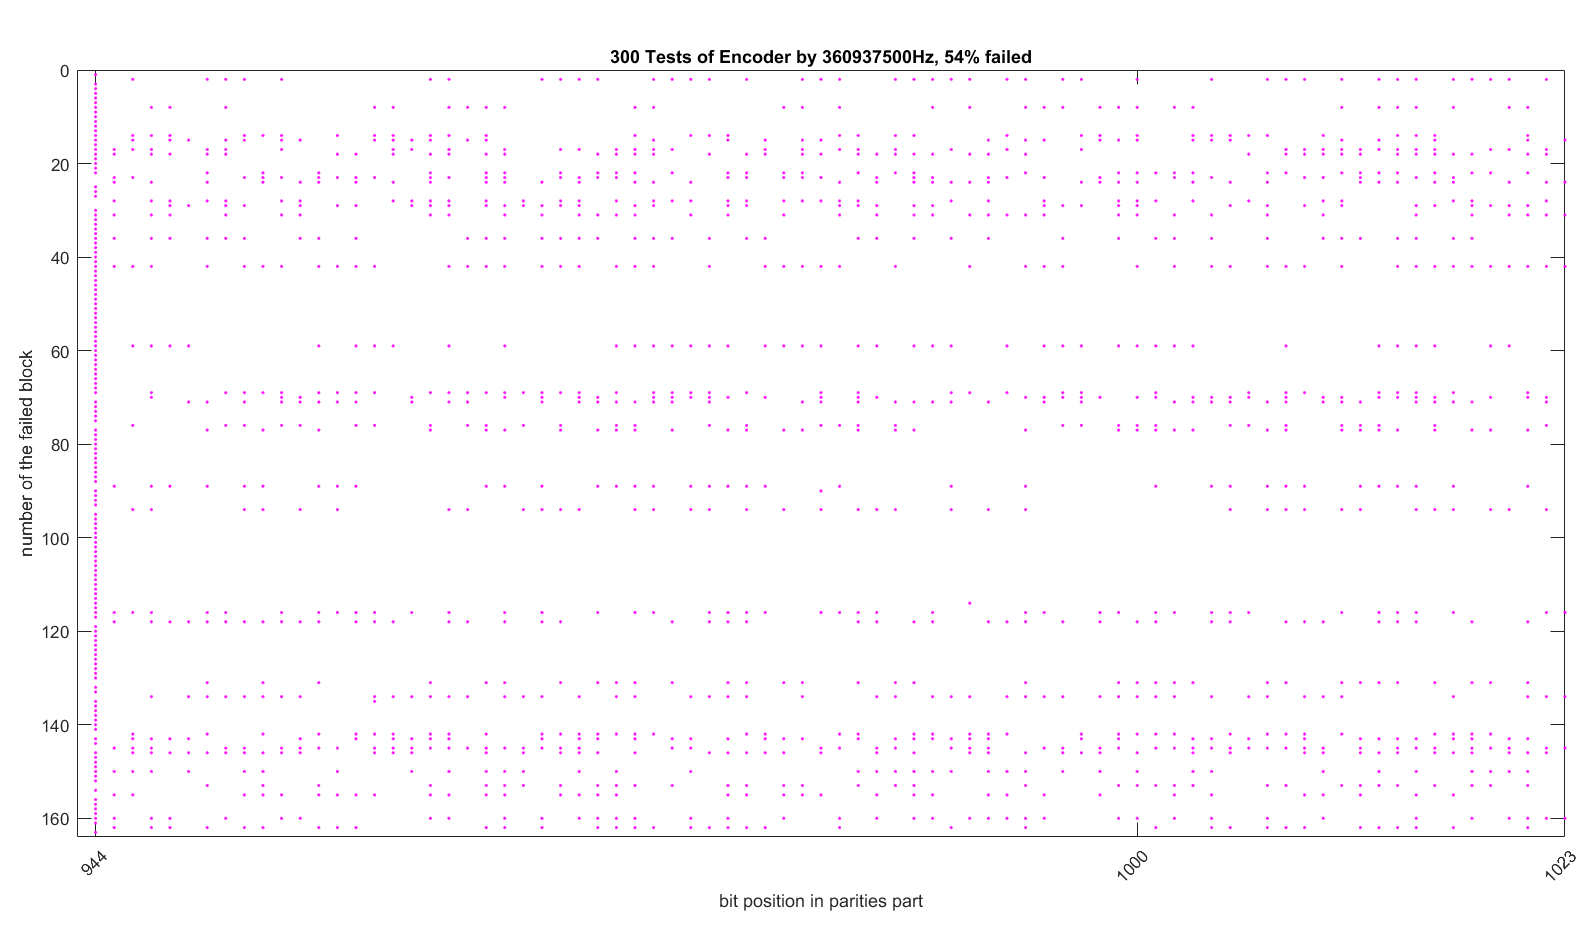
\includegraphics[width=\textwidth]{figures/test_ENC_multiple.png}
\caption{The result of failed Encoder test by 360 MHz}
\label{fig:enc_2}
\end{figure}

\section{Test of BCH(1023,943) Decoder}

The BCH(1023,943) allows a correction of 8 bits in one block. The PENCA architecture contains BCH codes being able to correct up to 15 bits in a single block. 
